% Generated from the accompanying manuscript.md by typeset.py.
\documentclass[11pt,a4paper]{article}
\usepackage[T1]{fontenc}
\usepackage[utf8]{inputenc}
\usepackage{lmodern}
\usepackage[a4paper,margin=25mm]{geometry}
\usepackage{amsmath,amssymb,amsthm}
\usepackage{microtype}
\usepackage{graphicx,longtable,booktabs,array,calc}
\usepackage[hidelinks,pdfencoding=auto,hypertexnames=false]{hyperref}
\hypersetup{
  pdftitle={Sharp density thresholds for finite two-visit scheduling},
  pdfauthor={Fabian Fetik}
}
\urlstyle{same}
\providecommand{\tightlist}{\setlength{\itemsep}{0pt}\setlength{\parskip}{0pt}}
\setlength{\emergencystretch}{1.5em}
\setlength{\LTpre}{0.7em}
\setlength{\LTpost}{0.7em}
\widowpenalty=10000
\clubpenalty=10000
\allowdisplaybreaks[1]
\title{Sharp density thresholds for finite two-visit scheduling}
\author{Fabian Fetik}
\date{}
\begin{document}
\maketitle
\begin{abstract}
In finite two-visit pinwheel scheduling, each of \(n\) labelled tasks with positive integer deadline \(d_i\) must occur exactly twice in a word of length \(2n\). Its first occurrence must be among the first \(d_i\) positions, and the two occurrences must be at most \(d_i\) positions apart. We prove that every instance of density \(\sum_i 1/d_i\le1\) is feasible, including equality. More sharply, for every fixed \(n\ge2\), all instances of density at most \(1+1/[n(n-1)]\) are feasible except relabellings of \((n-1,n,\ldots,n)\), and this exception is infeasible. A constructive anchor-cluster repair yields a schedule with linear combinatorial work after sorting and an exact density check. The proof combines an ordered reciprocal inequality with a calendar that controls the relative order of the two visits.
\end{abstract}
\hypertarget{introduction}{%
\section*{Introduction}\label{introduction}}

The finite \(k\)-Visits problem asks for exactly \(k\) occurrences of each task, with no deadline expiring before an initial or subsequent visit. It is distinct from perpetual pinwheel scheduling because tasks retire after their final occurrence. The original finite formulation and its computational complexity were studied by Kanellopoulos, Pergaminelis, Kokkou, Markou and Pagourtzis \cite{ref:KPK+26}. Kanellopoulos, Mitropoulos, Pergaminelis and Tolias \cite[Theorem 44]{ref:KMPT26} proved that density at most \(\sqrt2-1/2\) suffices for two visits. They bounded the lower density threshold between \(\sqrt2-1/2\) and one, and identified one as a possible exact value \cite[Section 8]{ref:KMPT26}. We prove that one is the exact universal guarantee, including equality, and determine the minimum infeasible density for each fixed task count.

Our construction begins with the latest allowed primary positions, which we call anchors, as in the position-matching formulation of Kanellopoulos et al. \cite{ref:KPK+26}. Consecutive blocks of anchors form clusters; the unused positions serve as partners for the other visit of each label. Pairing anchors and partners in sorted order can fail even on feasible inputs. We preserve the positions assigned to each cluster and repair its matching with an auxiliary calendar whose capacity records the long deadlines. An ordered reciprocal inequality rules out every late calendar completion at density one. For density slightly above one, a quantitative margin handles large prefixes; a structural reduction leaves four small patterns, all repaired by the same calendar.

Formally, an input is a labelled list of positive integers \(d_1,\ldots,d_n\). A feasible word occupies every slot in \([2n]=\{1,\ldots,2n\}\) and contains each label twice. If its two positions are \(p_i<q_i\), feasibility means \(p_i\le d_i\) and \(q_i-p_i\le d_i\). Labels with equal deadlines remain distinct. This is equivalent to the primary/secondary formulation of Kanellopoulos et al.~\cite{ref:KMPT26}: a designated primary position \(a_i\le d_i\) and another position \(v_i\le a_i+d_i\) yield a legal chronological pair in either order; conversely, the first chronological visit can be designated primary. There is no wraparound constraint.

\begin{quote}
\begin{minipage}{\linewidth}
\textbf{Theorem A (universal threshold).} Every finite labelled integer-deadline 2-Visits instance with \(D=\sum_i1/d_i\le1\) has a feasible word. The infimum of densities of infeasible instances is one, but no infeasible instance has density one.
\end{minipage}
\end{quote}

\begin{quote}
\begin{minipage}{\linewidth}
\textbf{Theorem B (fixed-count threshold).} For every \(n\ge2\), an \(n\)-task instance with \(D\le\alpha_n:=1+1/[n(n-1)]\) has a feasible word unless its multiset of deadlines is \(B_n=(n-1,n,\ldots,n)\). The multiset \(B_n\) is infeasible. Thus \(\alpha_n\) is the exact minimum infeasible density at fixed \(n\), with a unique minimizer up to relabelling.
\end{minipage}
\end{quote}

\begin{quote}
\begin{minipage}{\linewidth}
\textbf{Corollary C (construction).} There is an algorithm that, for every input covered by Theorem B, either constructs a feasible word or identifies the exception \(B_n\). It uses \(O(n\log n)\) deadline comparisons and \(O(n)\) further scheduling operations, with \(O(n)\) combinatorial working storage. The exact rational density comparison has polynomial bit complexity and is accounted for separately.
\end{minipage}
\end{quote}

For a fixed task count, Theorem B guarantees feasibility below \(\alpha_n\) and classifies infeasibility at equality. Thus \(\alpha_n\) is a minimum infeasible density. Theorem A gives the universal lower density threshold in the terminology of Kanellopoulos et al.~\cite{ref:KMPT26}.

The general 2-Visits decision problem is strongly NP-complete, as proved by Kanellopoulos et al.~\cite{ref:KPK+26}. Corollary C concerns the specified density region; an input above \(\alpha_n\) can be feasible or infeasible, and the algorithm makes no decision for that region. The empty input and a single task are immediate.

\hypertarget{proof-overview}{%
\subsection*{Proof overview}\label{proof-overview}}

The main difficulty is that a short deadline may require a different order of tasks in the anchor positions and in their complementary partner positions. A single sorted order cannot always satisfy both. Our repair controls the difference between these two orders while preserving the positions assigned to each cluster.

Sections 2--3 remove tasks that can be appended, choose distinct anchors, and isolate a failed cluster. The first few partner positions precede the cluster and can retain their sorted labels. The remaining labels divide into short tasks, with deadlines \(K-\delta_j\), and long tasks, with deadlines \(K+c_\ell\). The nonincreasing lengths \(\delta_j\) measure the advancement needed by short tasks; the nondecreasing capacities \(c_\ell\) measure the additional delay allowed to long tasks.

Sections 4--6 place these short lengths in an auxiliary calendar. Its capacity at column \(\ell\) is \(c_\ell\). Raising the availability cuts keeps job starts and ends ordered, and the resulting artificial idle time has a telescoping bound. If a job completed too late, that bound would limit the total long-task capacity. The ordered reciprocal inequality would then force density greater than one. Section 7 turns the calendar into two permutations: a short task is inserted after its end in the anchor order and after its start in the partner order. This advances it by exactly \(\delta_j\), while a long task is delayed by at most \(c_\ell\). Section 7.3 gives an eight-task example of the complete repair.

For Theorem B, each failed cluster is charged to a prefix of \(M\le n\) tasks that preserves its assigned positions. Section 8 strengthens the density contradiction to \(D>1+1/(12M)\), which exceeds the allowed margin when \(M\ge13\). Section 9 handles \(M\le12\) by an analytic reduction to four short-job patterns and proves that the same calendar repairs all four. Section 10 combines these repairs and the exceptional family. The entire argument concerns the finite first-visit and gap conditions stated above.

\hypertarget{sharpness-and-the-exact-finite-contract}{%
\section{Sharpness and the exact finite contract}\label{sharpness-and-the-exact-finite-contract}}

Repeated deadlines always denote different labels. There is one label in every position, no wraparound requirement, and no obligation after a label's second visit. These are the finite-model conventions of \cite{ref:KPK+26,ref:KMPT26}.

For \(B_n\), all deadlines are at most \(n\). Every label must therefore receive its first visit in the first \(n\) positions. Those positions contain exactly the \(n\) first visits, and positions \(n+1,\ldots,2n\) contain exactly the second visits. In any such word,
\[
\sum_i(q_i-p_i)
=\sum_{t=n+1}^{2n}t-\sum_{t=1}^n t=n^2.
\]

But
\[
\sum_i d_i=(n-1)+(n-1)n=n^2-1.
\]

Thus at least one gap exceeds its deadline, proving \(B_n\) infeasible. Its density is \(\alpha_n\) and tends to one from above. Together with feasibility at density at most one, proved below, this establishes Theorem A's sharpness.

\hypertarget{anchor-positions-and-the-reduction-to-individual-clusters}{%
\section{Anchor positions and the reduction to individual clusters}\label{anchor-positions-and-the-reduction-to-individual-clusters}}

We use the primary-position construction of the position-matching formulation \cite{ref:KPK+26}, and call its designated positions \textbf{anchors}. An anchor may be either the first or the second chronological visit of its label.

\hypertarget{appendable-tasks-and-positive-anchor-positions}{%
\subsection{Appendable tasks and positive anchor positions}\label{appendable-tasks-and-positive-anchor-positions}}

Deleting both visits of any label and compressing preserves all remaining inequalities. Conversely, an \(n\)-task input with a task of deadline at least \(2n-1\) can append that task at positions \(2n-1,2n\) after a solution for the other tasks.

Sort deadlines nondecreasingly, and repeatedly remove the largest task whenever its deadline is at least \(2n-1\), with \(n\) the current task count. Removed tasks will be appended in reverse removal order. Density cannot increase. It is enough to solve the resulting core. If the core is nonempty, it has \(n\ge2\) and maximum deadline at most \(2n-2\). All notation below refers to this core until the removed tasks are restored.

Density at most one implies \(d_i\ge i\) for every sorted index \(i\), since
\[
1\ge D\ge\sum_{r=1}^i\frac1{d_r}\ge\frac{i}{d_i}.
\]

Define
\begin{equation}
a_n=d_n,\qquad a_i=\min(d_i,a_{i+1}-1)\quad(i=n-1,\ldots,1).
\tag{2.1}
\label{eq:2.1}
\end{equation}

Backward induction gives \(i\le a_i\le d_i\). Thus the anchors \(A=\{a_1<\cdots<a_n\}\) are distinct positions in \([1,2n]\). Let their complement be
\begin{equation}
v_1<\cdots<v_n,\qquad \{v_1,\ldots,v_n\}=[1,2n]\setminus A.
\tag{2.2}
\label{eq:2.2}
\end{equation}

A labelled pair \((a,v)\), with \(a\le d\) and \(v\le a+d\), is legal: if \(v>a\), its first visit is \(a\) and its gap is at most \(d\); if \(v<a\), its first visit is \(v<a\le d\) and its gap is less than \(a\le d\).

\hypertarget{clusters-and-a-sufficient-sorted-pairing}{%
\subsection{Clusters and a sufficient sorted pairing}\label{clusters-and-a-sufficient-sorted-pairing}}

A cluster is a maximal consecutive block of anchors. Write one cluster as the indices \(p+1,\ldots,q\), and put
\[
b=a_q=d_q,\qquad H=b-q.
\]

The equality \(a_q=d_q\) follows immediately from \eqref{eq:2.1} at a cluster boundary, or from \(a_n=d_n\) at the last cluster. Within the cluster,
\begin{equation}
a_i=H+i\quad(p<i\le q).
\tag{2.3}
\label{eq:2.3}
\end{equation}

Assign this cluster the partner positions \(v_{p+1},\ldots,v_q\). Distinct clusters use disjoint anchor and partner positions. Therefore independent legal pairings for all clusters combine into one word.

The sorted pairing \((d_i,a_i,v_i)\) works for a cluster whenever
\begin{equation}
v_i\le a_i+d_i\quad(p<i\le q).
\tag{2.4}
\label{eq:2.4}
\end{equation}

We retain the sorted pairs for every passing cluster and construct legal pairings on the same assigned positions for every cluster where \eqref{eq:2.4} fails. Combining these pairings will give the required word.

\hypertarget{density-accounting-for-a-failed-cluster}{%
\section{Density accounting for a failed cluster}\label{density-accounting-for-a-failed-cluster}}

Fix a cluster where \eqref{eq:2.4} fails. Since the partner positions are gaps, a failed partner must lie beyond the end of the cluster. Thus \(v_q>b\). Set
\begin{equation}
T=v_q,\qquad t=T-2q,\qquad c=2H-t,\qquad K=q-H+t.
\tag{3.1}
\label{eq:3.1}
\end{equation}

There are exactly \(q\) partner positions at or before \(T\), hence \(T-q=q+t\) anchors there. All of the first \(q\) anchors precede \(T\), so \(t\ge0\) counts the additional anchors encountered before the last partner assigned to the present cluster.

When \(t>0\), because \(T\) is a gap, the last of these additional anchors ends its cluster. Consequently all tasks with indices \(q+1,\ldots,q+t\) have deadlines less than \(T\). Their density is at least \(t/T\); these tasks are disjoint from the first \(q\) tasks.

In particular,
\begin{equation}
D\ge\frac q b+\frac tT,
\qquad
\frac q b+\frac tT-1=\frac{q(t-2H)}{bT}.
\tag{3.2}
\label{eq:3.2}
\end{equation}

Thus \(c\ge0\). If \(c=0\), then \(K=b\) and the lower bound in \eqref{eq:3.2} equals one. A failed index satisfies
\begin{equation}
d_i<v_i-a_i\le T-(q-i)-(H+i)=K=b,
\tag{3.3}
\label{eq:3.3}
\end{equation}

so the first \(q\) tasks have density strictly greater than \(q/b\), contradicting \(D\le1\). Therefore
\begin{equation}
c\ge1.
\tag{3.4}
\label{eq:3.4}
\end{equation}

The useful parameter identities are
\begin{equation}
H=\frac{c+t}{2},\qquad b=K+c,\qquad T=2K+c,
\qquad k:=q-H=K-t.
\tag{3.5}
\label{eq:3.5}
\end{equation}

\hypertarget{a-local-half-density-bound}{%
\subsection{A local half-density bound}\label{a-local-half-density-bound}}

Among the first \(q\) tasks, let \(S\) be the density of those whose deadline is at most \(K\), and let \(R_0\) be their number. Since \(R_0\le KS\),
\[
D\ge S+\frac{q-R_0}{b}+\frac tT
\ge\frac q b+\frac c b S+\frac tT.
\]

Combining this with \(D\le1\) and \eqref{eq:3.5} yields the exact estimate
\begin{equation}
\boxed{S\le\frac qT\le\frac12.}
\tag{3.6}
\label{eq:3.6}
\end{equation}

A failed index has deadline less than \(K\), by \eqref{eq:3.3}. If \(H\le p\), all the first \(p\) tasks are among those counted by \(S\), and the preceding cluster boundary gives
\[
d_p=a_p\le a_{p+1}-2=H+p-1.
\]

Here \(H\ge1\), because \(c\ge1\) and \(H\) is an integer. Hence
\[
S\ge\frac p{H+p-1}>\frac12,
\]

a contradiction. We have proved
\begin{equation}
H>p.
\tag{3.7}
\label{eq:3.7}
\end{equation}

There are exactly \(H=b-q\) gaps before the end of the cluster, and there are no gaps inside it. A failed index therefore exceeds \(H\). Let
\[
R=\max\{i\le q:d_i<K\},\qquad h=R-H.
\]

Then \(h\ge1\), and \(R<q\), since \(d_q=b>K\). The remaining \(k=q-H\) labels divide into
\begin{equation}
\begin{aligned}
&\text{short labels: } H+j,
&&a'_j:=d_{H+j}=K-\delta_j,
&&1\le j\le h,\\
&\text{long labels: } R+\ell,
&&d_{R+\ell}=K+c_\ell,
&&1\le\ell\le L:=k-h.
\end{aligned}
\tag{3.8}
\label{eq:3.8}
\end{equation}

Thus
\begin{equation}
\delta_1\ge\cdots\ge\delta_h\ge1,
\qquad
0\le c_1\le\cdots\le c_L=c,
\qquad L\ge1.
\tag{3.9}
\label{eq:3.9}
\end{equation}

The short lengths and long capacities retain all their distinct values.

\hypertarget{the-reciprocal-inequality-used-in-the-repair}{%
\section{The reciprocal inequality used in the repair}\label{the-reciprocal-inequality-used-in-the-repair}}

The main density estimate is the following reciprocal inequality. It applies to real parameters \(c,t,K\) in the stated ranges, with \(H=(c+t)/2\).

\hypertarget{lemma-4.1.-ordered-reciprocal-inequality}{%
\subsection*{Lemma 4.1. Ordered reciprocal inequality}\label{lemma-4.1.-ordered-reciprocal-inequality}}

Let \(c\ge1\), \(t\ge0\), and an integer \(j\ge1\) be given. Set
\[
H=(c+t)/2,\quad K\ge c+t+j,\quad L'=K-t-j,
\quad B=K^2+(2c-t-1)K+c^2,\quad T=2K+c.
\]

For \(j=1\) and \(0<x\le K\),
\begin{equation}
\frac{H+1}{x}+\frac{(L')^2}{B-2cx}+\frac tT>1.
\tag{4.1}
\label{eq:4.1}
\end{equation}

For \(j\ge2\) and \(0<x\le y\le K\),
\begin{equation}
\frac{H+1}{x}+\frac{j-1}{y}
+\frac{(L')^2}{B-(c+1)x-(c+j-2)y}
+\frac tT>1.
\tag{4.2}
\label{eq:4.2}
\end{equation}

All displayed denominators are positive: the denominator involving \(B\) is at least \(KL'+c^2>0\), and \(L'\ge c>0\).

\hypertarget{step-1-respect-the-ordering-before-applying-cauchy}{%
\subsection*{Step 1: respect the ordering before applying Cauchy}\label{step-1-respect-the-ordering-before-applying-cauchy}}

For \(j\ge2\), abbreviate
\[
P=H+1,\quad J=j-1,\quad u=c+1,\quad V=c+j-2.
\]

When \(PV\ge Ju\), write \(x=s y\), \(0<s\le1\). Then
\[
\left(\frac P x+\frac J y\right)(ux+Vy)
 -(P+J)(u+V)
=(1-s)\left(\frac{PV}{s}-Ju\right)\ge0.
\]

Putting \(a=(ux+Vy)/(u+V)\le K\), the first three terms in \eqref{eq:4.2} are therefore at least
\begin{equation}
f(a)=\frac{H+j}{a}
       +\frac{(L')^2}{B-(2c+j-1)a}.
\tag{4.3}
\label{eq:4.3}
\end{equation}

The case \(j=1\) has this form directly, with \(a=x\). Weighted Cauchy gives the further, unrestricted lower bound
\begin{equation}
f(a)\ge\frac{(L'+S_{\rm p}(j))^2}{B},
\qquad S_{\rm p}(j)=\sqrt{(H+j)(2c+j-1)}.
\tag{4.4}
\label{eq:4.4}
\end{equation}

When \(PV<Ju\), Cauchy applied instead to the denominators \(ux,Vy,B-ux-Vy\) gives a lower bound of the same form with
\begin{equation}
S_{\rm f}(j)=\sqrt{(H+1)(c+1)}
             +\sqrt{(j-1)(j+c-2)}.
\tag{4.5}
\label{eq:4.5}
\end{equation}

We use these unrestricted bounds only in the parameter range where they suffice.

\hypertarget{step-2-one-positive-seed-for-0le-tle3c-2}{%
\subsection*{\texorpdfstring{Step 2: one positive seed for \(0\le t\le3c-2\)}{Step 2: one positive seed for 0\textbackslash le t\textbackslash le3c-2}}\label{step-2-one-positive-seed-for-0le-tle3c-2}}

For any \(\rho\), define
\begin{equation}
N(K,\rho)
=(2K+c)(K+\rho-t)^2
 -(2K+c-t)[K^2+(2c-t-1)K+c^2].
\tag{4.6}
\label{eq:4.6}
\end{equation}

If \(\rho=S-j\), then \((L'+S)^2/B+t/T>1\) is exactly \(N(K,\rho)>0\). Put
\[
w=\sqrt{1+(t+2)/c}-1,\qquad
\rho_1=c(1+w)-1=S_{\rm p}(1)-1.
\]

Here \(0<w\le1\) and \(\rho_1>0\). For \(z=K-c-t-1\ge0\), direct expansion gives
\begin{equation}
N(K,\rho_1)=N_0+N_1z+Az^2,
\tag{4.7}
\label{eq:4.7}
\end{equation}

where
\begin{equation}
\begin{aligned}
A&=cw(2-w)>0,\\
N_1&=c^2(4w+w^2-w^4)+c(w-1)^2>0,\\
N_0&=c^3(2w+2w^2-w^4)+c^2(w-1)^2>0.
\end{aligned}
\tag{4.8}
\label{eq:4.8}
\end{equation}

The signs follow from \(0<w\le1\); for example \(w^4\le w^2\). Moreover,
\begin{equation}
\partial_\rho N(K,\rho)=2(2K+c)(K+\rho-t)>0
\quad(K>t,\ \rho\ge0).
\tag{4.9}
\label{eq:4.9}
\end{equation}

It consequently suffices, at every \(j\), to show \(S-j\ge\rho_1\).

For the pooled value, the function \(\rho_{\rm p}(v)=\sqrt{(H+v)(2c+v-1)}-v\) is nondecreasing for real \(v\ge1\): its derivative is the arithmetic mean of the two positive factors divided by their geometric mean, minus one. Hence \(S_{\rm p}(j)-j\ge\rho_{\rm p}(1)=\rho_1\).

For the free value, its regime condition is equivalent to
\[
(c-t)(j-1)>(c-1)(c+t+2).
\]

It implies \(t<c\), and therefore \(t\le3c-2\). Define
\begin{equation}
j_0=1+\frac{(c-1)(c+t+2)}{c-t}\ge1.
\tag{4.10}
\label{eq:4.10}
\end{equation}

The free regime has \(j>j_0\). At \(j_0\), the two Cauchy values agree, because \(PV=Ju\). The function
\[
\rho_{\rm f}(v)
=\sqrt{(H+1)(c+1)}+\sqrt{(v-1)(v+c-2)}-v
\]

is nondecreasing for \(v>j_0\), again by arithmetic mean versus geometric mean. It is continuous at \(j_0\); for \(c=1,j_0=1\), the last square root equals \(v-1\). Thus
\[
S_{\rm f}(j)-j\ge\rho_{\rm f}(j_0)
=\rho_{\rm p}(j_0)\ge\rho_1.
\]

Since \(K\ge c+t+j\ge c+t+1\), \eqref{eq:4.7}--\eqref{eq:4.9} prove the desired strict inequality in every uncapped case.

\hypertarget{step-3-preserve-the-cap-when-tge3c-2}{%
\subsection*{\texorpdfstring{Step 3: preserve the cap when \(t\ge3c-2\)}{Step 3: preserve the cap when t\textbackslash ge3c-2}}\label{step-3-preserve-the-cap-when-tge3c-2}}

For \(j\ge2\), at the boundary \(t=3c-2\) we have \(PV-Ju=(c-1)(j+2c-1)\ge0\), and this expression increases with \(t\). Thus \eqref{eq:4.3} applies; for \(j=1\), it already applies directly. Write \(W=H+j\), \(v=2c+j-1\). Now \(W\ge v\). For \(0<a\le K\),
\[
B-va=KL'+c^2+v(K-a)\ge aL',
\qquad
f'(a)=-\frac W{a^2}
       +\frac{v(L')^2}{(B-va)^2}\le0.
\]

Hence \(f(a)\ge f(K)\). The required endpoint value has the identity
\begin{equation}
f(K)+\frac tT-1
=\frac{c}{2K}
 \left(\frac{T-t}{T}-\frac{2cL'}{KL'+c^2}\right).
\tag{4.11}
\label{eq:4.11}
\end{equation}

All denominators are positive. Also \(K\ge c+t+j\ge4c-1\ge3c\), and \(t\le K-c-j\). Consequently
\begin{equation}
\begin{aligned}
K(T-t)-2cT
&=(K-2c)T-Kt\\
&\ge(K-2c)T-K(K-c-j)\\
&=(K-3c)(K+c)+c^2+jK>0.
\end{aligned}
\tag{4.12}
\label{eq:4.12}
\end{equation}

The numerator of the parenthesis in \eqref{eq:4.11}, after multiplying by \(T(KL'+c^2)\), is
\[
L'[K(T-t)-2cT]+c^2(T-t)>0.
\]

This proves the capped case and completes the lemma. \(\square\)

\hypertarget{an-auxiliary-calendar-with-bounded-idle-time}{%
\section{An auxiliary calendar with bounded idle time}\label{an-auxiliary-calendar-with-bounded-idle-time}}

Return to the failed cluster's short lengths \(\delta_j\) and long capacities \(c_\ell\) from \eqref{eq:3.8}--\eqref{eq:3.9}. Imagine long-label columns \(1,\ldots,L\), with \(c_\ell\) available machines in column \(\ell\). Machine \(u\), for \(1\le u\le c\), becomes available at column
\[
\lambda_u=\min\{\ell:c_\ell\ge u\}.
\]

It exists because \(c_L=c\). A machine's availability is stored as a \textbf{cut}: initially \(r_u=\lambda_u-1\). A job of length \(\delta\) assigned after cut \(r\) occupies columns \(r+1,\ldots,r+\delta\) and ends at cut \(r+\delta\). For the moment extend the calendar indefinitely, keeping all \(c\) machines available beyond column \(L\). We will prove that the jobs actually used all end before \(L\).

Process the short jobs in their order \(1,\ldots,h\). Let \(e_0=0\). At job \(j\):

\begin{enumerate}
\def\labelenumi{\arabic{enumi}.}
\tightlist
\item
  Replace every availability cut \(r_u\) by \(\max(r_u,e_{j-1}-\delta_j)\). Count each increase as artificial idle time.
\item
  Choose a machine with minimum availability cut, breaking ties by machine index. Put the job there and set \(e_j=r_u+\delta_j\); update that machine's availability to \(e_j\).
\end{enumerate}

Let \(s_j=e_j-\delta_j\) be the job's starting cut. By construction,
\begin{equation}
e_1\le\cdots\le e_h,
\qquad s_1\le\cdots\le s_h.
\tag{5.1}
\label{eq:5.1}
\end{equation}

The second assertion uses the nonincreasing sequence \(\delta_j\). Jobs on the same machine do not overlap. Hence at every column \(\ell\) the number of jobs with \(s_j<\ell\le e_j\) is at most \(c_\ell\).

\hypertarget{lemma-5.1.-total-artificial-idle-time}{%
\subsection*{Lemma 5.1. Total artificial idle time}\label{lemma-5.1.-total-artificial-idle-time}}

Just before placing job \(j\), the total artificial idle time inserted on all machines is at most
\begin{equation}
c(\delta_1-\delta_j).
\tag{5.2}
\label{eq:5.2}
\end{equation}

\textbf{Proof.} After job \(j-1\), every availability cut is at least \(e_{j-1}-\delta_{j-1}\). To raise one to \(e_{j-1}-\delta_j\) costs at most \(\delta_{j-1}-\delta_j\). There are \(c\) machines. No idle time is needed at the first step, and the sum telescopes. The stated lower bound on all cuts holds inductively because the chosen cut is the minimum and the chosen job ends exactly \(\delta_j\) later. \(\square\)

The raising step keeps the starts and ends ordered even when the lengths vary. Its total cost is bounded by the drop from the first length to the current length.

\hypertarget{every-calendar-completion-is-early-enough}{%
\section{Every calendar completion is early enough}\label{every-calendar-completion-is-early-enough}}

We prove
\begin{equation}
\boxed{e_j\le a'_j-2H-j=K-\delta_j-2H-j
\quad(1\le j\le h).}
\tag{6.1}
\label{eq:6.1}
\end{equation}

\hypertarget{a-preliminary-separation-forced-by-density}{%
\subsection{A preliminary separation forced by density}\label{a-preliminary-separation-forced-by-density}}

For a fixed \(j\), all the first \(H+j\) deadlines are at most \(a'_j=K-\delta_j\), and all the other deadlines among the first \(q\) are at most \(b=K+c\). Thus
\begin{equation}
\frac{H+j}{K-\delta_j}
 +\frac{K-t-j}{K+c}+\frac t{2K+c}\le D\le1.
\tag{6.2}
\label{eq:6.2}
\end{equation}

Writing \(\delta=\delta_j\), multiply the left side minus one by its positive common denominator \(2(K+c)(K-\delta)(2K+c)\). The numerator is
\begin{equation}
\begin{aligned}
P(K)={}&-2cK^2\\
&+K(c^2+4c\delta+4cj+3ct+4\delta j+2\delta t)\\
&+c^3+2c^2\delta+2c^2j+c^2t+2c\delta j.
\end{aligned}
\tag{6.3}
\label{eq:6.3}
\end{equation}

It has exactly one positive root: its leading coefficient is negative and its constant and linear coefficients are positive. At \(K_*=c+t+j+2\delta\),
\begin{equation}
P(K_*)=(c+2\delta)
 (3cj+ct+4\delta j+2\delta t+2j^2+3jt+t^2)>0.
\tag{6.4}
\label{eq:6.4}
\end{equation}

Inequality \eqref{eq:6.2} therefore implies
\begin{equation}
K>c+t+j+2\delta_j.
\tag{6.5}
\label{eq:6.5}
\end{equation}

In particular, the domain \(K\ge c+t+j\) of Lemma 4.1 is available, and the prefix length used next is positive.

\hypertarget{a-missed-completion-bound-limits-the-total-capacity}{%
\subsection{A missed completion bound limits the total capacity}\label{a-missed-completion-bound-limits-the-total-capacity}}

Suppose \eqref{eq:6.1} fails for some \(j\), and put
\[
U=K-\delta_j-2H-j,
\qquad X=U-\delta_j+1
       =K-c-t-j-2\delta_j+1>0.
\]

Just before job \(j\) is placed, after raising the cuts, their minimum is \(e_j-\delta_j>U-\delta_j\). All cuts are integral, so every cut is at least \(X\). The available machine area through column \(X\) must consequently be accounted for by the first \(j-1\) jobs and the artificial idle time. More explicitly, if machine \(u\) has processed work \(W_u\) and received artificial idle time \(I_u\), its current cut is \(\lambda_u-1+W_u+I_u\ge X\). Thus \(\max(0,X-\lambda_u+1)\le W_u+I_u\). Summing over machines and using Lemma 5.1 gives
\begin{equation}
\sum_{\ell=1}^X c_\ell
\le\sum_{i<j}\delta_i+c(\delta_1-\delta_j).
\tag{6.6}
\label{eq:6.6}
\end{equation}

Here \(c_\ell=c\) for \(\ell>L\), as stipulated in the extended calendar. Let \(C=\sum_{\ell=1}^L c_\ell\). If \(X\le L\), bound the remaining columns by \(c\); if \(X>L\), subtract the exactly constant extension. In either case,
\begin{equation}
\begin{aligned}
C
&\le\sum_{i<j}\delta_i+c(\delta_1-\delta_j)+c(L-X)\\
&=\sum_{i<j}\delta_i+c^2+c(\delta_1+\delta_j)+c(j-h-1)\\
&\le C_*:=\sum_{i<j}\delta_i+c^2+c(\delta_1+\delta_j).
\end{aligned}
\tag{6.7}
\label{eq:6.7}
\end{equation}

The area in \eqref{eq:6.6} counts the full capacity profile from \eqref{eq:3.9}, so \eqref{eq:6.7} bounds the sum of the original long-task capacities.

\hypertarget{the-capacity-bound-contradicts-density}{%
\subsection{The capacity bound contradicts density}\label{the-capacity-bound-contradicts-density}}

The first \(H\) tasks contribute at least \(H/a'_1\). The first \(j\) short tasks contribute their actual reciprocals. The remaining \(h-j\) short tasks have deadlines at most \(K\). Cauchy applied to those tasks together with all long tasks gives
\begin{equation}
D\ge
\frac{H+1}{a'_1}+\sum_{i=2}^j\frac1{a'_i}
+\frac{(K-t-j)^2}{K(K-t-j)+C}+\frac tT.
\tag{6.8}
\label{eq:6.8}
\end{equation}

For clarity, this Cauchy step first uses \(\sum_{\ell=1}^L1/(K+c_\ell)\ge L^2/(KL+C)\), and then combines this with \((h-j)/K\). Their combined number is \(L+h-j=K-t-j\).

Replace \(C\) by the upper bound \(C_*\), which only decreases the right side. Let \(B\) be as in Lemma 4.1.

For \(j=1\),
\[
K(K-t-1)+C_*=B-2ca'_1,
\]

so \eqref{eq:6.8} exceeds one by \eqref{eq:4.1}, a contradiction.

For \(j\ge2\), put
\[
x=a'_1,\qquad y=\frac1{j-1}\sum_{i=2}^j a'_i.
\]

Then \(0<x\le y<K\), and
\[
\sum_{i=2}^j\frac1{a'_i}\ge\frac{j-1}{y}.
\]

Also
\begin{equation}
\begin{aligned}
K(K-t-j)+C_*
&=B-(c+1)a'_1-\sum_{i=2}^{j-1}a'_i-ca'_j\\
&\le B-(c+1)x-(c+j-2)y.
\end{aligned}
\tag{6.9}
\label{eq:6.9}
\end{equation}

The last step follows from \(a'_j\ge y\) and \(c\ge1\). The right side of \eqref{eq:6.8} is therefore at least the left side of \eqref{eq:4.2}, which is strictly greater than one. This contradiction proves \eqref{eq:6.1} for every \(j\).

\hypertarget{reconstruction-of-the-original-word}{%
\section{Reconstruction of the original word}\label{reconstruction-of-the-original-word}}

We now recover a word on the cluster's assigned positions.

For the labels \(p+1,\ldots,H\), use the sorted pairs \((a_i,v_i)\). Their partner positions precede the entire cluster, while \(a_i\le d_i\); hence these pairs are legal.

The remaining anchors are exactly
\[
2H+1,\ldots,b,
\]

and the remaining partner positions are
\[
v_{H+1},\ldots,v_q.
\]

Make two permutations \(P,Q\) of the \(k\) remaining labels. Keep the long labels in increasing order in both. Insert short label \(j\) after \(e_j\) long labels in \(P\), and after \(s_j=e_j-\delta_j\) long labels in \(Q\). For ties use increasing short index. Both insertions are ordered by \eqref{eq:5.1}. They lie within the long-label range: \eqref{eq:6.1} at \(j=h\) gives
\[
e_h\le K-\delta_h-2H-h=L-c-\delta_h<L.
\]

Place \(P\) into anchors \(2H+1,\ldots,b\), and \(Q\) into partner positions \(v_{H+1},\ldots,v_q\). All these partners follow \(b\). Since they are increasing integral positions ending at \(T\),
\begin{equation}
v_{H+r}\le b+t+r\quad(1\le r\le k).
\tag{7.1}
\label{eq:7.1}
\end{equation}

A label whose ranks in the two permutations are \(r_P,r_Q\) has gap at most
\begin{equation}
b+t+r_Q-(2H+r_P)=K+r_Q-r_P.
\tag{7.2}
\label{eq:7.2}
\end{equation}

For short label \(j\), its ranks are \(e_j+j\) and \(s_j+j\), so its gap is at most \(K-\delta_j=a'_j\). Its first position is
\[
2H+e_j+j\le a'_j
\]

by \eqref{eq:6.1}.

For long label \(\ell\), a short job precedes it in \(Q\) exactly when \(s_j<\ell\), and in \(P\) exactly when \(e_j<\ell\). Thus the difference \(r_Q-r_P\) counts precisely the jobs with \(s_j<\ell\le e_j\), and is at most \(c_\ell\). Its gap is therefore at most \(K+c_\ell=d_{R+\ell}\). Its first position is at most
\[
2H+h+\ell=a_{R+\ell}\le d_{R+\ell}.
\]

Thus every repaired pair satisfies the two original inequalities. Performing this repair separately on each failed cluster, retaining every passing sorted cluster, gives a word covering every one of the \(2n\) core positions exactly once. Restore the appendable tasks as in Section 2.1. This proves the universal theorem, including \(D=1\). \(\square\)

\hypertarget{a-geometric-calendar-and-a-linear-time-sweep}{%
\subsection{A geometric calendar and a linear-time sweep}\label{a-geometric-calendar-and-a-linear-time-sweep}}

The machine calendar admits an equivalent description with no machine identities or artificial-idle bookkeeping in the implementation.

Extend the capacity profile by \(c_\ell=c\) after column \(L\), as before. Suppose the previous ends \(e_1\le\cdots\le e_{j-1}\) have been placed. For the next width \(\delta_j\), choose the smallest integer cut
\begin{equation}
s\ge\max(0,e_{j-1}-\delta_j)
\quad\text{such that}\quad
c_{s+1}\ge1+\#\{i<j:e_i>s\}.
\tag{7.3}
\label{eq:7.3}
\end{equation}

Put \(s_j=s\) and \(e_j=s+\delta_j\), with \(e_0=0\). The condition has a solution: take \(s\) after all prior ends and after all machines have become available. Because previous starts are at most the candidate \(s\), their occupancy cannot increase after column \(s+1\), whereas capacity cannot decrease. Thus the displayed one-column test ensures that the whole new interval fits the geometric capacity profile.

\textbf{Lemma 7.1 (equivalence of the two calendars).} Rule \eqref{eq:7.3} produces exactly the ends and starts of Section 5, for every nondecreasing integral capacity profile ending at \(c\ge1\) and every nonincreasing positive integral width list.

\textbf{Proof.} At step \(j\), write \(f=e_{j-1}-\delta_j\). The successive values of this lower bound are nondecreasing. On each machine, after the raising operation its cut is the maximum of its release cut, its last actual job end if any, and \(f\). This description follows by induction from the raising and assignment operations; it also covers unused machines.

For any candidate \(s\ge\max(0,f)\), that machine is available at or before \(s\) exactly when it has been released by column \(s+1\) and has no prior job ending after \(s\). The first step is immediate. For \(j\ge2\), all prior starts are at most \(s\), because
\[
s\ge e_{j-1}-\delta_j
\ge e_{j-1}-\delta_{j-1}=s_{j-1}.
\]

Consequently each prior end greater than \(s\) corresponds to one occupied, released machine, and no two such jobs can use the same machine. The number of machines free by \(s\) is exactly \(c_{s+1}-\#\{i<j:e_i>s\}\). The first cut admitting a free machine is therefore exactly \eqref{eq:7.3}. The minimum-cut machine rule of Section 5 chooses the same cut. Induction proves equality of all ends and starts. \(\square\)

By this lemma, \eqref{eq:6.1} applies unchanged to \eqref{eq:7.3}. In particular every end is less than \(L\).

To implement \eqref{eq:7.3}, maintain a nondecreasing cut \(s\) and a pointer \(z\) counting prior ends at most \(s\):

\noindent\begin{minipage}{\linewidth}
\begin{verbatim}
ends := empty list; s := 0; z := 0
for each width delta in nonincreasing order:
    s := max(s, last(ends, default=0) - delta)
    while true:
        while z < len(ends) and ends[z] <= s:
            z := z + 1
        if capacity[s+1] >= 1 + len(ends) - z:
            break
        s := s + 1
    append s + delta to ends
\end{verbatim}
\end{minipage}

For clarity, \texttt{ends} uses zero-based array indices in this pseudocode, while \texttt{capacity} uses the mathematical one-based column index. The cut never moves backwards, and it remains below \(L\) under the theorem's hypothesis. Across the entire cluster there are at most \(L\) failed candidate tests and at most \(h\) successful ones. The pointer advances at most \(h\) times. Thus this calendar takes \(O(L+h)\) operations. The two permutations are made by linear merges of the already ordered ends or starts with the long-label columns.

\hypertarget{constructivity-and-boundary-cases}{%
\subsection{Constructivity and boundary cases}\label{constructivity-and-boundary-cases}}

After sorting the original deadlines, preprocessing, anchors, complement positions, cluster identification, the geometric sweeps, reconstruction and original-word verification all take \(O(n)\) operations on \(O(\log n)\)-bit core positions, aside from reading and comparing the original deadline values. The sums of \(L+h\) and of cluster sizes over distinct clusters are at most \(n\). Locating \(R\) can be done by a backward scan within the current cluster, since \(R>H>p\); repeatedly scanning the full prefix is unnecessary.

Thus the implementation uses \(O(n\log n)\) comparisons for unsorted input and linear additional scheduling work, or linear scheduling work on already sorted input. These operation counts exclude the exact rational check \(D\le1\); that check has polynomial bit complexity in the input's binary encoding length. All subsequent numerical work in the core is bounded by \(O(n)\)-sized integers. The entire algorithm has polynomial bit work and \(O(n)\) combinatorial working storage.

The empty input needs no word. A one-task input is handled by the appendable rule. The density check uses the original deadlines. Labels are mapped back to their input identities after sorting, preserving distinct labels with repeated numerical deadlines.

\hypertarget{an-eight-task-repair}{%
\subsection{An eight-task repair}\label{an-eight-task-repair}}

Let the labels be \(A,B,C,D,E,F,G,H\), with respective deadlines \((6,6,9,9,9,9,9,9)\). The density is exactly \(2/6+6/9=1\). To distinguish the label \(H\) from the cluster parameter, write \(H_{\rm cl}\) for that parameter in this example. The anchors and partners are
\[
(a_1,\ldots,a_8)=(2,3,4,5,6,7,8,9),\qquad
(v_1,\ldots,v_8)=(1,10,11,12,13,14,15,16).
\]

They form one anchor cluster, with \(p=0,q=8,b=9,H_{\rm cl}=1,T=16,t=0,c=2,K=7\). The sorted pairing assigns \(B\) to positions \(3,10\), whose gap is seven and exceeds its deadline six. The pair for \(A\) occupies positions \(2,1\) and is already legal; we leave it there.

Among the remaining labels, only \(B\) is short: \(\delta_1=K-d_B=1\). The six long labels \(C,\ldots,H\) all have capacity \(c_\ell=9-K=2\). The calendar places the unit job for \(B\) in its first column, with \(s_1=0,e_1=1\). Its completion satisfies the required bound \(e_1=1\le K-\delta_1-2H_{\rm cl}-1=3\). The two permutations are consequently
\[
P=(C,B,D,E,F,G,H),\qquad Q=(B,C,D,E,F,G,H).
\]

Place \(P\) at anchors \(3,\ldots,9\) and \(Q\) at partners \(10,\ldots,16\). Together with the retained pair for \(A\), this gives the word
\[
A\ A\ C\ B\ D\ E\ F\ G\ H\ B\ C\ D\ E\ F\ G\ H.
\]

The complete position check is small enough to display:

\begin{center}
\begin{tabular}{@{}lrrrr@{}}
\toprule\noalign{}
Label & Deadline & First position & Second position & Gap \\
\midrule\noalign{}


\(A\) & 6 & 1 & 2 & 1 \\
\(B\) & 6 & 4 & 10 & 6 \\
\(C\) & 9 & 3 & 11 & 8 \\
\(D\) & 9 & 5 & 12 & 7 \\
\(E\) & 9 & 6 & 13 & 7 \\
\(F\) & 9 & 7 & 14 & 7 \\
\(G\) & 9 & 8 & 15 & 7 \\
\(H\) & 9 & 9 & 16 & 7 \\
\bottomrule
\end{tabular}
\end{center}

Every first position and gap is within its deadline. In the two orders, \(B\) has \(r_Q-r_P=-1\), reducing its gap to \(K-1=6\). Label \(C\) has \(r_Q-r_P=1\), increasing its gap to \(K+1=8\), within its capacity allowance. All other long labels have zero rank difference. Figure 1 shows the changed positions and the calendar interval.

\begin{figure}
\centering
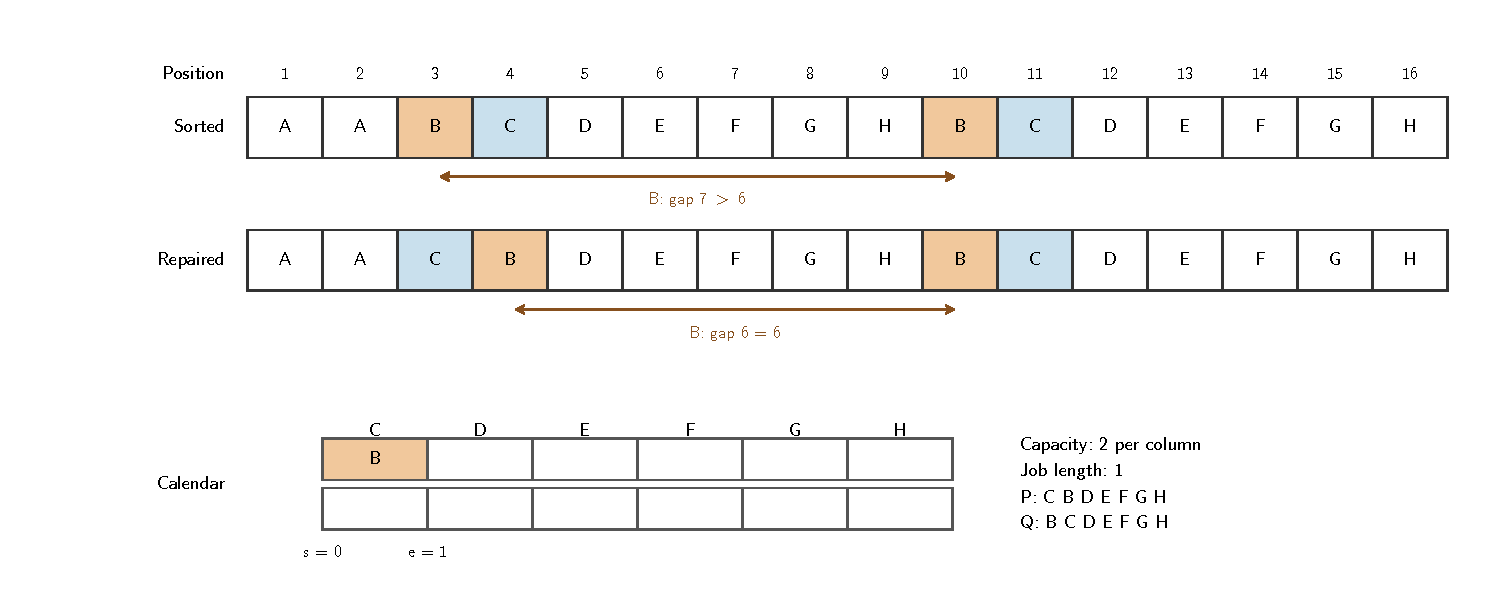
\includegraphics[width=\linewidth]{figures/repair-example.pdf}
\caption{Repair of the eight-task example. The sorted word gives B a gap of seven; the repaired word gives B a gap of six. The unit calendar job crosses column C, delaying C by one rank, within the two available capacity units.}
\end{figure}

\hypertarget{fixed-count-extension-and-quantitative-margin}{%
\section{Fixed-count extension and quantitative margin}\label{fixed-count-extension-and-quantitative-margin}}

\hypertarget{proof-strategy}{%
\subsection{Proof strategy}\label{proof-strategy}}

We strengthen the calendar estimate by a uniform margin, then apply it to large charged prefixes. Small prefixes are resolved analytically in Section 9.

\hypertarget{a-quantitative-reciprocal-inequality-on-the-integer-lattice}{%
\subsection{A quantitative reciprocal inequality on the integer lattice}\label{a-quantitative-reciprocal-inequality-on-the-integer-lattice}}

\textbf{Lemma 8.1.} In Lemma 4.1, additionally suppose that \(c\ge1\) and \(t\ge0\) are integers and \(c+t\) is even. Thus \(H=(c+t)/2\) is an integer at least one. Set \(M=K+H\). Each applicable left side of \eqref{eq:4.1} or \eqref{eq:4.2} is strictly greater than
\begin{equation}
1+\frac1{12M}.
\tag{8.1}
\label{eq:8.1}
\end{equation}

The domains for \(x,y,j,K\) are otherwise exactly those of Lemma 4.1. In particular, \(K\ge c+t+j=2H+j\); the lemma does not require an original input or an actual failed calendar.

\textbf{Proof, uncapped range.} Suppose \(t\le3c-2\). The ordered pooling, Cauchy, and monotonicity arguments of Section 4 give the lower bound
\[
\frac{(K+R-1-t)^2}{B}+\frac tT,
\quad
R=\sqrt{c(c+t+2)}=\sqrt{2c(H+1)},
\quad T=2K+c.
\]

These arguments cover both the pooled and the free Cauchy regimes: their respective values of \(S-j\) are at least \(R-1\). Let
\[
N=T(K+R-1-t)^2-(T-t)B,
\qquad b=K+c,
\qquad z=K-2H-1\ge0.
\]

The range assumptions give \((H+1)/2\le c\le2H\). The chord estimate
\begin{equation}
R\ge\frac{2(c+H+1)}3
\tag{8.2}
\label{eq:8.2}
\end{equation}

follows by squaring, since
\[
9R^2-4(c+H+1)^2
=2(2c-H-1)(2H+2-c)\ge0.
\]

After using \(R^2=2c(H+1)\), \(N\) is affine in \(R\). Its coefficient of \(R\) is
\[
4z^2+(8H+6c+4)z+c(8H+2c+4)>0.
\]

Substitution of \eqref{eq:8.2}, with \(c=2H-t\), therefore yields
\begin{equation}
N\ge\frac Q3,
\quad
Q=(t+2)z^2+2((H-1)t+5H+1)z+c(t^2+6H+2).
\tag{8.3}
\label{eq:8.3}
\end{equation}

There is the exact identity
\begin{equation}
2Q-b^2=(2t+3)z^2+((4H-2)t+12H+2)z+C,
\tag{8.4}
\label{eq:8.4}
\end{equation}

where
\[
C=8H^2+4Ht^2-4Ht-2t^3-t^2-2t-1.
\]

If \(t=0\), then \(C=8H^2-1>0\). Otherwise the integer \(t\) is at least one. Put
\[
u=H-\frac{2t+1}{3}\ge0,\qquad v=t-1\ge0;
\]

the first inequality follows from \(t\le3c-2\) and \(c=2H-t\). Direct substitution gives
\begin{equation}
C=8u^2+4uv^2+\frac{44}{3}uv+16u
 +\frac23v^3+\frac{29}{9}v^2+\frac{14}{3}v+2>0.
\tag{8.5}
\label{eq:8.5}
\end{equation}

All coefficients of \(z\) in \eqref{eq:8.4} are positive. Hence \eqref{eq:8.3}--\eqref{eq:8.5} imply \(6N>b^2\). Finally,
\[
B=b^2-(t+1)K<b^2,\qquad T=2M-t\le2M.
\]

Consequently the excess above one of the Cauchy lower bound satisfies
\[
\frac{N}{BT}>\frac1{6T}\ge\frac1{12M}.
\]

This proves the uncapped range.

\textbf{Proof, capped range.} Suppose \(t\ge3c-2\). The capped argument in Section 4 shows that the expression is at least \(f(K)+t/T\). With \(L'=K-t-j>0\), equation \eqref{eq:4.11} gives its excess over one as
\[
\frac{c}{2K}
\left(\frac{T-t}{T}-\frac{2cL'}{KL'+c^2}\right).
\]

Since \(t\le K-c-j\le K-c-1\), the expression in parentheses is strictly larger than
\[
\frac{K+2c+1}{2K+c}-\frac{2c}{K}.
\]

This last expression exceeds \(1/6\). To see this, multiply its difference from \(1/6\) by the positive number \(6K(2K+c)\). The numerator is
\[
4K^2+(6-13c)K-12c^2.
\]

We have \(K\ge4c-1\). Substituting \(w=K-(4c-1)\ge0\) transforms the numerator into
\[
4w^2+(19c-2)w+5c-2>0.
\]

Thus the excess is greater than \(c/(12K)\), which is greater than \(1/(12M)\). This proves the lemma. \(\square\)

The distinction \(t=0\) or \(t\ge1\) in \eqref{eq:8.5} uses integrality. Thus the quantitative margin of Lemma 8.1 applies to the integer parameters of an input, whereas Lemma 4.1 applies to the broader real-parameter domain.

\hypertarget{a-failed-cluster-has-a-controlled-reusable-prefix}{%
\subsection{A failed cluster has a controlled, reusable prefix}\label{a-failed-cluster-has-a-controlled-reusable-prefix}}

We now prove Theorem B. First prove it for appendage-free cores at their own task counts. Deleting an appendable task strictly lowers density, and \(\alpha_r>\alpha_n\) for \(2\le r<n\). Therefore a proper remaining core of an input with density at most \(\alpha_n\) has density strictly less than its own \(\alpha_r\), cannot be its critical exception, and can be restored by Section 2.1. Cores of size zero or one are immediate.

Let the core have size \(n\), density \(D\le\alpha_n\), and not be \(B_n\). If \(d_i<i\), then
\[
D\ge\frac i{i-1}\ge1+\frac1{n-1}>\alpha_n.
\]

Thus all anchors remain positive, with \(a_i\ge i\), even though the present density hypothesis is greater than one.

Consider a cluster rejected by the sorted rule. Retain \(p,q,b,H,T,t,c,K\) from Sections 2--3 and add
\begin{equation}
M=q+t=K+H.
\tag{8.6}
\label{eq:8.6}
\end{equation}

There are precisely \(M\) anchors before the gap \(T=v_q\). The last of them ends a cluster, so
\[
d_M=a_M<T,\qquad M\le n.
\]

Also \(T=2M-t\) and \(b=M+H-t\). The failed partner lies after the cluster; since there are \(H\) gaps before its end, \(H<q\). In particular \(b<2q\le2M\). A failed cluster cannot have \(M=1\): that would give \(q=1,t=H=0,d_1=a_1=1,T=2\), which passes the sorted test.

\textbf{Prefix stability.} Truncate the deadline list after index \(M\). Its anchor recurrence starts at \(d_M=a_M\), so all its anchors agree with the first \(M\) original anchors. Its first \(q\) partner positions also agree with the original ones, because \(T\le2M\) and the two anchor sets agree at all positions at most \(T\).

The prefix's maximum deadline is at most \(2M-2\). If \(t>0\), this follows from \(d_M<T=2M-t\). If \(t=0\), the only possible larger value is \(d_M=2M-1\). That would mean \(M=q\) and \(H=M-1\), leaving only index \(q\) with a partner after the cluster. But its deadline and anchor are both \(2M-1\), and its partner is \(2M\), so it does not fail. This contradicts the choice of the cluster.

The prefix has density at most the core density, so \(D_{\mathrm{prefix}}\le D\le\alpha_n\le\alpha_M\). It cannot equal \(B_M\): if \(M<n\), that prefix alone would already have density \(\alpha_M>\alpha_n\), while if \(M=n\), it would be the excluded original exception \(B_n\).

If \(M\le12\), the prefix is handled by the small-prefix repair of Section 9. That repair uses only the labels, anchors and partners assigned to the rejected cluster. Since these positions agree with those in the original core, we can insert its repaired pairs directly into that core.

It remains to solve rejected clusters with \(M\ge13\). For these,
\begin{equation}
D\le\alpha_n\le\alpha_M\le1+\frac1{12M}.
\tag{8.7}
\label{eq:8.7}
\end{equation}

\hypertarget{the-structural-inequalities-still-hold-above-density-one}{%
\subsection{The structural inequalities still hold above density one}\label{the-structural-inequalities-still-hold-above-density-one}}

The accounting identity \eqref{eq:3.2} is independent of the density-one hypothesis:
\begin{equation}
D\ge\frac q b+\frac tT
=1-\frac{qc}{bT}.
\tag{8.8}
\label{eq:8.8}
\end{equation}

\textbf{First, \(c\ge1\).} If \(c\le-1\), then \(b<2q\) gives
\[
D>1+\frac1{2T}\ge1+\frac1{4M}>\alpha_M,
\]

contradicting \eqref{eq:8.7}. If \(c=0\), a failed index has \(d_i<K=b\), while all first \(q\) deadlines are at most \(b\). The lower bound in \eqref{eq:8.8} equals one, and integrality gives the additional reciprocal cost
\begin{equation}
D\ge1+\frac1{b(b-1)}.
\tag{8.9}
\label{eq:8.9}
\end{equation}

Here \(b\ge2\), since a positive deadline is less than \(b\). Also \(c=0\) gives \(t=2H\) and \(b=M-H\le M\). If \(b<M\), \eqref{eq:8.9} strictly exceeds \(\alpha_M\). Otherwise \(b=M\), so \(H=t=0\) and \(q=M\). Equality with the allowed density can hold only when \(M=n\), exactly one deadline is \(n-1\), and all others are \(n\): any extra task, a second decreased deadline, or a further decrease makes \eqref{eq:8.9} strict. This is precisely the excluded \(B_n\). Thus \(c\ge1\), and \(H\ge1\).

\textbf{Second, \(H>p\).} Let \(S\) be the density of first-\(q\) deadlines at most \(K\), as in Section 3.1. The same counting, without imposing \(D\le1\), gives
\begin{equation}
D-1\ge\frac cb\left(S-\frac qT\right).
\tag{8.10}
\label{eq:8.10}
\end{equation}

Suppose \(H\le p\). The failed deadline is less than \(K\), so all the first \(p\) deadlines are counted by \(S\). The preceding cluster boundary gives \(d_p\le H+p-1\), and therefore
\begin{equation}
S\ge\frac p{H+p-1}\ge\frac H{2H-1},
\quad
D-1\ge\frac{c}{2b}
 \left(\frac1{2H-1}+\frac tT\right).
\tag{8.11}
\label{eq:8.11}
\end{equation}

If \(t=0\), then \(c=2H\) and the right side exceeds \(1/(2b)>1/(4M)>\alpha_M-1\). If \(t\ge1\), put \(s=2H-1=c+t-1\). Since \(c,t\) are positive integers, \(ct\ge c+t-1=s\). Arithmetic mean versus geometric mean now gives
\[
D-1\ge\frac1{2b}\left(\frac1s+\frac sT\right)
\ge\frac1{b\sqrt T}
>\frac1{2M\sqrt{2M}}
>\frac1{M(M-1)}.
\]

The final strict inequality holds for \(M\ge13\), because \((M-1)^2-8M=(M-13)^2+16(M-13)+40>0\). Again this contradicts \(D\le\alpha_M\). Thus \(H>p\).

We may consequently define the same short labels, positive widths \(\delta_j\), and nondecreasing long capacities \(c_\ell\) as in \eqref{eq:3.8}--\eqref{eq:3.9}, retaining their actual values.

\hypertarget{quantitative-preliminary-separation}{%
\subsection{Quantitative preliminary separation}\label{quantitative-preliminary-separation}}

To use the area argument above density one, we strengthen the separation estimate \eqref{eq:6.5} by a quantitative density contradiction.

For a short label \(j\), its actual anchor bound is
\[
K-\delta_j=d_{H+j}\ge a_{H+j}=2H+j.
\]

Put \(r=K-2H-j\); then \(r\ge\delta_j\ge1\). Suppose the desired separation fails, so \(r\le2\delta_j\). The density estimate \eqref{eq:6.2} is increasing with \(\delta_j\), and \(\delta_j\ge r/2\). Set \(K=2H+j+r\) and \(M=3H+j+r\). It follows that
\begin{equation}
D-1\ge
\frac{(c+r)[jM+t(H+r/2)]}
 {(K+c)(K-r/2)T}.
\tag{8.12}
\label{eq:8.12}
\end{equation}

This identity is also obtained by substituting \(\delta=r/2\) into the cleared numerator in \eqref{eq:6.4}.

Write \(U=2H+r\), so \(c+r=U-t\ge2\) and \(U+j<M<3U/2+j\). The numerator in \eqref{eq:8.12} is
\[
A=(U-t)(jM+tU/2).
\]

We claim \(A>(2/9)M^2\). If \(t=0\), then \(A=UjM\), and
\[
Uj>U/3+2j/9>2M/9.
\]

The first inequality uses \(U\ge3,j\ge1\); the second uses \(M<3U/2+j\). If \(t\ge1\), let \(a=U-t\ge2\). Then \(at\ge a+t-1=U-1\), and
\[
A\ge2jM+(U-1)U/2
>2j(U+j)+(U^2-U)/2.
\]

Subtracting \((2/9)(3U/2+j)^2\) from the last expression gives
\[
\frac43Uj+\frac{16}{9}j^2-\frac U2>0.
\]

This proves the claim in both cases. Meanwhile,
\[
K+c\le M+H<\frac43M,\quad K-r/2<M,\quad T\le2M.
\]

The denominator in \eqref{eq:8.12} is therefore less than \((8/3)M^3\). We obtain
\[
D-1>\frac1{12M},
\]

contradicting \eqref{eq:8.7}. Hence
\[
K>c+t+j+2\delta_j
\]

for every short label, as required.

\hypertarget{calendar-completion-reconstruction-and-equality-classification}{%
\subsection{Calendar completion, reconstruction, and equality classification}\label{calendar-completion-reconstruction-and-equality-classification}}

Use the same unequal-length calendar as in Section 5, or its equivalent linear sweep in Section 7.1. The artificial-idle bound of Lemma 5.1 is independent of density. If a completion bound \eqref{eq:6.1} fails, the preceding separation ensures \(X>0\), and the area argument \eqref{eq:6.6}--\eqref{eq:6.7} applies unchanged. So do the reciprocal lower bound \eqref{eq:6.8}, its ordered reduction \eqref{eq:6.9}, and positivity of all denominators.

Now Lemma 8.1 makes the resulting density lower bound strictly greater than \(1+1/(12M)\), contradicting \eqref{eq:8.7}. Thus every completion satisfies \eqref{eq:6.1}. The inequalities just established allow the reconstruction of Section 7, giving legal original pairs for this cluster, including every first-position deadline.

Every rejected cluster is therefore solved: by the analytic small-prefix repair when \(M\le12\), and by the quantitative calendar argument when \(M\ge13\). Passing clusters retain their sorted pairs. The clusters partition all labels, anchors, and partner positions, so their matchings give a full original word. Restore any deleted appendable tasks. This proves feasibility under \(D\le\alpha_n\) outside \(B_n\).

Section 1 proves \(B_n\) infeasible and computes its density as \(\alpha_n\). Thus there is no lower-density infeasible input at fixed \(n\), and the only infeasible input at the endpoint, up to relabelling, is \(B_n\). The small-prefix repair used here is proved in Section 9. With that lemma, this completes the proof of Theorem B. \(\square\)

\hypertarget{analytic-small-prefix-repair}{%
\section{Analytic small-prefix repair}\label{analytic-small-prefix-repair}}

\hypertarget{setup-and-a-sharper-structural-density-identity}{%
\subsection{Setup and a sharper structural density identity}\label{setup-and-a-sharper-structural-density-identity}}

Use the core, anchors, clusters, and partners of Sections 2 and 8.3. Consider a cluster rejected by the sorted pairing, with indices \(p+1,\ldots,q\), and put
\begin{equation}
b=H+q,\quad T=v_q,\quad t=T-2q,\quad
 M=q+t,\quad K=M-H,\quad c=2H-t.
\tag{9.1}
\label{eq:9.1}
\end{equation}

Thus \(b=K+c\), \(T=2M-t=2K+c\), and \(q=K+H-t\). As in Section 8.3, \(M\) counts exactly the anchors before the gap \(T\); truncation after \(M\) preserves the present cluster and all its assigned partners. In this section suppose \(M\le 12\). The prefix has density at most \(\alpha_M\), and is not \(B_M\), by the prefix argument of Section 8.3. Write \(D\) for its density; every lower bound below concerns only its actual tasks.

The anchors are positive, since the fixed-task density promise implies \(d_i\ge i\). Also \(H\ge 0\). A failed index must be greater than \(H\): there are exactly \(H\) gaps before the end of the cluster, and every such gap precedes the whole cluster. Therefore \(q>H\). All first \(q\) deadlines are at most \(b\). All the remaining \(t\) deadlines in the prefix are at most \(T-1\), since its last anchor ends a cluster strictly before the gap \(T\).

\textbf{First exclude \(H=0\).} Then the first \(q\) anchors are \(1,\ldots,q\) and \(d_q=q\). If \(t>0\),
\[
 D\ge1+\frac{t}{2M-t-1}
 \ge1+\frac1{2M-2}.
\]

For \(M>2\) this exceeds \(\alpha_M\). For \(M=2\), equality would force exactly \((1,2)=B_2\), already excluded. If \(t=0\), then \(q=M\) and a sorted-pair failure requires some deadline at most \(M-1\), while all deadlines are at most \(M\). Consequently \(D\ge \alpha_M\), with equality only for \(B_M\). Thus \(H\ge 1\).

\textbf{Next, \(c\ge 1\).} The exact accounting identity \eqref{eq:3.2} still gives
\begin{equation}
D\ge\frac qb+\frac tT=1-\frac{qc}{bT}.
\tag{9.2}
\label{eq:9.2}
\end{equation}

If \(c\le -1\), then \(t\ge 2H+1\), and \(q>H\) implies \(M=q+t\ge 3H+2\ge 5\). Since \(b=H+q<2q\),
\[
 D>1+\frac1{2T}\ge1+\frac1{4M}\ge\alpha_M,
\]

a contradiction. If \(c=0\), a failed deadline is strictly below \(K=b\). Integrality adds at least \(1/[b(b-1)]\) to the right side of \eqref{eq:9.2}, which is one. Here \(b=M-H<M\), so this again exceeds \(\alpha_M\). Thus \(c\ge 1\). In particular,
\begin{equation}
0\le t\le2H-1.
\tag{9.3}
\label{eq:9.3}
\end{equation}

A failed index has deadline less than \(K\), by \eqref{eq:3.3}. Hence at least the first \(H+1\) deadlines are at most \(K-1\). The last deadline of this cluster is \(b=K+c>K\), so there is at least one further task in it. We obtain
\begin{equation}
D\ge F(M,H,t):=
 \frac{H+1}{K-1}+\frac{K-t-1}{K+c}
 +\frac{t}{2M-t-1}.
\tag{9.4}
\label{eq:9.4}
\end{equation}

All denominators are positive and \(K-t-1\ge 1\). Put
\[
 F_0(M,H)=\frac{H+1}{M-H-1}
              +\frac{M-H-1}{M+H}.
\]

The following two identities bound \(H\) in terms of \(M\):
\begin{equation}
F(M,H,t)-F_0(M,H)
 =\frac{t(K-1)(K-t-1)}
 {(M+H)(M+H-t)(2M-t-1)}\ge0,
\tag{9.5}
\label{eq:9.5}
\end{equation}

and
\begin{equation}
F_0(M,H)-\alpha_M
 =\frac{H\bigl[(3H+4-M)M(M-1)+H+1\bigr]}
 {M(M-1)(M-H-1)(M+H)}.
\tag{9.6}
\label{eq:9.6}
\end{equation}

If \(M\le 3H+4\), \eqref{eq:9.6} is strictly positive. Therefore every failed cluster with \(c\ge 1\) under the fixed-task promise necessarily satisfies
\begin{equation}
\boxed{M\ge3H+5.}
\tag{9.7}
\label{eq:9.7}
\end{equation}

This implication itself is not restricted to small \(M\). For \(M\le 12\), it leaves only
\begin{equation}
H=1,\quad 8\le M\le12;
 \qquad\text{or}\qquad
 H=2,\quad 11\le M\le12.
\tag{9.8}
\label{eq:9.8}
\end{equation}

\hypertarget{no-later-anchor-interference-in-a-small-failed-cluster}{%
\subsection{No later-anchor interference in a small failed cluster}\label{no-later-anchor-interference-in-a-small-failed-cluster}}

Let
\[
 R=\max\{i\le q:d_i<K\},\qquad h=R-H\ge1,
 \qquad \delta_j=K-d_{H+j}\quad(1\le j\le h).
\]

The widths are positive and nonincreasing. These definitions do not yet require \(p<H\). For any \(j\le h\) with \(\delta_j\ge \delta\), counting the first \(H+j\) deadlines gives
\begin{equation}
D\ge G_{j,\delta}:=
 \frac{H+j}{K-\delta}+\frac{K-t-j}{K+c}
 +\frac t{2M-t-1}.
\tag{9.9}
\label{eq:9.9}
\end{equation}

Suppose \(t>0\). If \(h=1\) and \(\delta_1=1\), the only possible failed index is \(H+1\). It is in the cluster, and its partner is the first gap after the cluster, namely \(v_{H+1}=b+1\). Its anchor is \(2H+1\), so its actual gap is
\[
 b+1-(2H+1)=K-t\le K-1=d_{H+1}.
\]

All other potentially late partners have deadlines at least \(K\) and pass \eqref{eq:3.3}'s weak upper bound. Thus the cluster would not fail. A failed cluster with \(t>0\) must instead have either \(h\ge 2\) or \(\delta_1\ge 2\), forcing \(D\ge G_{2,1}\) or \(D\ge G_{1,2}\).

We show that both bounds exceed \(\alpha_M\) throughout \eqref{eq:9.8}. First,
\begin{equation}
G_{1,2}-G_{2,1}
 =\frac{(H-c)K+c(H+3)+2}{(K-2)(K-1)(K+c)}.
\tag{9.10}
\label{eq:9.10}
\end{equation}

For \(H=1\), necessarily \(t=c=1\), and the numerator is six. For \(H=2\), \(t=1,2,3\) and \(K=9,10\); the respective numerators are \(17-K\), \(12\), and \(K+7\), all positive. It is enough to consider \(G_{2,1}\).

For \(H=t=1\), direct simplification gives
\begin{equation}
G_{2,1}-\alpha_M
 =\frac{-M^2+14M-12}{2M(M-1)(M-2)}>0
 \quad(8\le M\le12),
\tag{9.11}
\label{eq:9.11}
\end{equation}

because its numerator \(M(14-M)-12\) is at least \(8*2-12>0\).

For \(H=2\), write \(G(t)\) for \(G_{2,1}\). For \(1\le t\le 3\),
\begin{equation}
G(t)-G(1)=(t-1)
 \left[
 \frac{2M-1}{(2M-t-1)(2M-2)}
 -\frac6{(M+2-t)(M+1)}
 \right].
\tag{9.12}
\label{eq:9.12}
\end{equation}

The bracket is at least
\[
 \frac{2M-1}{4(M-1)^2}-\frac6{(M-1)(M+1)}
 =\frac{2M^2-23M+23}{4(M-1)^2(M+1)}>0
 \quad(M\ge11).
\]

For the last sign, writing \(M=11+z\), \(z\ge 0\), makes its numerator \(12+21z+2z^2\). Finally, the only two relevant integer values give
\begin{equation}
G(1)-\alpha_{11}=\frac9{220}>0,
 \qquad
 G(1)-\alpha_{12}=\frac{107}{5148}>0.
\tag{9.13}
\label{eq:9.13}
\end{equation}

Equations \eqref{eq:9.10}--\eqref{eq:9.13} contradict either way in which a sorted failure with \(t>0\) could occur. We have proved
\begin{equation}
\boxed{t=0,\quad q=M,\quad c=2H.}
\tag{9.14}
\label{eq:9.14}
\end{equation}

\hypertarget{the-small-failed-cluster-is-the-first-cluster}{%
\subsection{The small failed cluster is the first cluster}\label{the-small-failed-cluster-is-the-first-cluster}}

We next show \(p=0\); no earlier cluster can consume some of the useful early positions. Suppose first that \(p\ge H\). Let \(S\) be the density of the first \(q\) tasks with deadlines at most \(K\), as in Section 3.1. Since a deadline in the present cluster is less than \(K\), every first-\(p\) deadline is counted by \(S\). The preceding cluster ends at deadline at most \(H+p-1\). Thus
\[
 S\ge\frac p{H+p-1}\ge\frac H{2H-1}.
\]

Use \eqref{eq:8.10}, now with \(t=0\), \(c=2H\), \(q/T=1/2\):
\[
 D-1\ge\frac{2H}{b}(S-1/2)
 \ge\frac{H}{b(2H-1)}
 >\frac1{2b}>\frac1{4M}>\alpha_M-1.
\]

The last inequality holds since \(M\ge 8\). Hence \(p<H\). If \(H=1\), this already says \(p=0\). If \(H=2\), the only other possibility is \(p=1\), which would give \(d_1\le 2\). Every other prefix deadline is at most \(b=M+2\), so
\[
 D\ge\frac12+\frac{M-1}{M+2}
 \ge\frac{33}{26}>\alpha_{11}\ge\alpha_M,
\]

again impossible. Therefore \(p=0\). The entire charged prefix consists of one anchor cluster, with anchors \(H+1,\ldots,M+H\) and partners \(1,\ldots,H,M+H+1,\ldots,2M\).

\hypertarget{only-four-short-job-patterns-remain}{%
\subsection{Only four short-job patterns remain}\label{only-four-short-job-patterns-remain}}

With \(t=0\), the lower bound \eqref{eq:9.9} satisfies
\begin{equation}
G_{j,\delta}-1
 =\frac{3H^2-HM+2Hj+2H\delta+j\delta}
 {(M-H-\delta)(M+H)}.
\tag{9.15}
\label{eq:9.15}
\end{equation}

\textbf{When \(H=1\).} If \(h\ge 3\), use \((j,\delta)=(3,1)\). If \(\delta_1\ge 3\), use \((1,3)\). In either case the numerator in \eqref{eq:9.15} is \(14-M\ge 2\), and its positive denominator is less than \(M(M-1)\). Both possibilities therefore force \(D>\alpha_M\).

It remains to exclude simultaneous \(h\ge 2\) and \(\delta_1\ge 2\). The first two deadlines are then at most \(K-2\), the third is at most \(K-1\), and all others are at most \(K+2\). Hence
\[
 D\ge F_{\rm mix}(M):=
 \frac2{M-3}+\frac1{M-2}+\frac{M-3}{M+1}.
\]

The identity
\begin{equation}
F_{\rm mix}(M)-1
 =\frac{11-M}{(M-2)(M+1)}
  +\frac2{(M-3)(M-2)}
\tag{9.16}
\label{eq:9.16}
\end{equation}

makes this strictly greater than \(\alpha_M-1\) for \(8\le M\le 11\). At \(M=12\), the exact excess is
\[
 F_{\rm mix}(12)-\alpha_{12}=\frac{179}{25740}>0.
\]

Consequently the only possible width lists for \(H=1\) are \((1)\), \((2)\), and \((1,1)\).

\textbf{When \(H=2\).} If \(h\ge 2\), use \((j,\delta)=(2,1)\) in \eqref{eq:9.15}. If \(\delta_1\ge 2\), use \((1,2)\). The numerator in both cases is \(26-2M\ge 2\), and the positive denominator is less than \(M(M-1)\). Again either assumption contradicts the density promise. Thus the sole possible width list is \((1)\).

The reduction is complete:

\begin{center}
\begin{tabular}{@{}
  >{\raggedright\arraybackslash}p{(\columnwidth - 6\tabcolsep) * \real{0.2308}}
  >{\raggedleft\arraybackslash}p{(\columnwidth - 6\tabcolsep) * \real{0.3077}}
  >{\raggedright\arraybackslash}p{(\columnwidth - 6\tabcolsep) * \real{0.2308}}
  >{\raggedright\arraybackslash}p{(\columnwidth - 6\tabcolsep) * \real{0.2308}}@{}}
\toprule\noalign{}
\begin{minipage}[b]{\linewidth}\raggedright
Pattern
\end{minipage} & \begin{minipage}[b]{\linewidth}\raggedleft
\(H\)
\end{minipage} & \begin{minipage}[b]{\linewidth}\raggedright
Width list
\end{minipage} & \begin{minipage}[b]{\linewidth}\raggedright
\(K\) range implied by the prefix size
\end{minipage} \\
\midrule\noalign{}


A & 1 & \((1)\) & \(7\le K\le11\) \\
B & 1 & \((2)\) & \(7\le K\le11\) \\
C & 1 & \((1,1)\) & \(7\le K\le11\) \\
D & 2 & \((1)\) & \(9\le K\le10\) \\
\bottomrule
\end{tabular}
\end{center}

The table contains every possible pattern under the density promise. The following argument repairs all four throughout the indicated ranges.

\hypertarget{the-same-calendar-succeeds-for-all-four-patterns}{%
\subsection{The same calendar succeeds for all four patterns}\label{the-same-calendar-succeeds-for-all-four-patterns}}

Use the original nondecreasing integral long capacities \(0\le c_1\le \ldots\le c_L=2H\). We prove the full completion bound \eqref{eq:6.1}, including its initial-position allowance, for the calendar of Sections 5 and 7.1.

For a \textbf{single short job of width \(\delta\)}, there are \(L=K-1\) long labels. Put
\[
 X=K-2\delta-2H.
\]

In patterns A, B, and D, \(X\ge 1\). If some capacity is positive in the first \(X\) columns, let \(r\le X\) be its first positive column. The calendar places this job with starting cut \(r-1\) and completion
\[
 e_1=r-1+\delta
 \le K-\delta-2H-1,
\]

which is exactly \eqref{eq:6.1}.

If instead all first \(X\) capacities vanish, their deadlines equal \(K\). The remaining \(L-X\) long deadlines are at most \(K+2H\), and the first \(H+1\) deadlines are at most \(K-\delta\). Therefore
\begin{equation}
D\ge\frac{H+1}{K-\delta}+\frac XK
                +\frac{L-X}{K+2H}.
\tag{9.17}
\label{eq:9.17}
\end{equation}

These expressions give the bad-capacity lower bounds \(F_A,F_B,F_D\) used below.

For \textbf{pattern C}, both jobs have width one. They are placed into the first two available units of column capacity: the monotone-start and monotone-end requirements introduce no extra restriction for equal unit widths. Put \(U=K-5\ge 2\). If the first \(U\) columns contain at least two capacity units, then both completions are at most \(U\). This implies \eqref{eq:6.1} for job two, whose bound is \(K-5\), and for job one, whose bound is \(K-4\).

If their capacity sum is at most one, monotonicity and integrality imply that the first \(U-1\) capacities are zero and the \(U\)-th is at most one. Here \(L=K-2\), so \(L-U=3\). The first three deadlines are at most \(K-1\). Thus
\begin{equation}
D\ge\frac3{K-1}+\frac{K-6}{K}
                   +\frac1{K+1}+\frac3{K+2}.
\tag{9.18}
\label{eq:9.18}
\end{equation}

Write the four bad-capacity lower bounds as
\[
\begin{aligned}
F_A&=\frac2{K-1}+\frac{K-4}{K}+\frac3{K+2},\\
F_B&=\frac2{K-2}+\frac{K-6}{K}+\frac5{K+2},\\
F_C&=\frac3{K-1}+\frac{K-6}{K}+\frac1{K+1}+\frac3{K+2},\\
F_D&=\frac3{K-1}+\frac{K-6}{K}+\frac5{K+4}.
\end{aligned}
\]

Each is strictly greater than its applicable fixed-task threshold. The exact differences are
\begin{equation}
\begin{aligned}
F_A-\alpha_{K+1}
 &=\frac{K^2(K-3)+4K+10}{K(K-1)(K+1)(K+2)},\\
F_B-\alpha_{K+1}
 &=\frac{K^2(K-6)+18K+28}{K(K-2)(K+1)(K+2)},\\
F_C-\alpha_{K+1}
 &=\frac{K^2(K-3)+6K+14}{K(K-1)(K+1)(K+2)},\\
F_D-\alpha_{K+2}
 &=\frac{2[K^2(K-4)(K+1)+27K+24]}{K(K-1)(K+1)(K+2)(K+4)}.
\end{aligned}
\tag{9.19}
\label{eq:9.19}
\end{equation}

All denominators are positive. All numerator expressions are manifestly positive for the respective \(K\) ranges in Section 9.4. Equations \eqref{eq:9.17}--\eqref{eq:9.18} therefore cannot occur. Every calendar completion satisfies \eqref{eq:6.1}.

Use exactly the reconstruction of Section 7: early labels keep their sorted pairs, short labels are inserted after \(e_j\) long labels in the anchor permutation and after \(e_j-\delta_j\) in the partner permutation, and long labels remain ordered. The initial deadlines and successive gaps follow from the already proved \eqref{eq:6.1} and the column capacities. The reconstruction uses only the prescribed cluster's anchors, partners, and labels.

We have proved the required analytic small-prefix result.

\textbf{Lemma 9.1 (analytic small-prefix repair).} Every failed cluster with charged prefix size \(M\le 12\) arising under the fixed-task density promise, outside the critical family, has a legal repair by the same calendar used for the large prefixes. It preserves exactly that cluster's assigned anchors and partner positions. \(\square\)

\hypertarget{completion-of-the-fixed-count-proof-and-algorithm}{%
\section{Completion of the fixed-count proof and algorithm}\label{completion-of-the-fixed-count-proof-and-algorithm}}

For a failed cluster of a prefix of size \(M\le12\), Lemma 9.1 gives a cluster-respecting legal repair. For \(M\ge13\), the estimates of Section 8 force \(c\ge1\), \(H>p\), and the strict preliminary separation. The calendar area bound and Lemma 8.1 then exclude a late completion, so the reconstruction of Section 7 applies. Passing clusters use the sorted pairs; appendable tasks are restored in reverse deletion order. Hence every input covered by Theorem B other than \(B_n\) has a word. The sum-of-gaps argument in Section 1 proves that \(B_n\) is infeasible, completing Theorem B.

The constructor sorts deadlines, deletes appendable tasks, builds anchors and partners, and sweeps each failed cluster with rule \eqref{eq:7.3}. The sweeps and reconstruction take linear combinatorial work after sorting. The exact rational comparison with the density promise has polynomial bit complexity. For \(B_n\), it supplies the explicit sum-of-gaps obstruction. The accompanying independent verifier checks the output word against the original first-visit and gap constraints, including repeated numerical deadlines as distinct labels. The operation and bit-complexity bounds in Section 7.2 apply to the same sweep under the fixed-count promise, establishing Corollary C.

\textbf{Use of AI tools.} ChatGPT and Codex were used to develop and review proof arguments and verification software, and to prepare this manuscript. The construction algorithm and the source code for the stated checks are supplied for independent verification.

\textbf{License.} This article is licensed under \href{https://creativecommons.org/licenses/by/4.0/}{CC BY 4.0}. The supplied Python software is licensed under MIT.
\begin{thebibliography}{KPK+26}
\bibitem[KPK+26]{ref:KPK+26}
Sotiris Kanellopoulos, Christos Pergaminelis, Maria Kokkou, Euripides Markou, and Aris Pagourtzis. \emph{Finite Pinwheel Scheduling: the k-Visits Problem}. In \emph{Proceedings of the 2026 Annual ACM-SIAM Symposium on Discrete Algorithms (SODA)}, pages 355--371, 2026. \href{https://doi.org/10.1137/1.9781611978971.16}{doi:10.1137/1.9781611978971.16}. \href{https://arxiv.org/abs/2507.11681v4}{Full version, arXiv:2507.11681v4}.
\bibitem[KMPT26]{ref:KMPT26}
Sotiris Kanellopoulos, Giorgos Mitropoulos, Christos Pergaminelis, and Thanos Tolias. \emph{Hardness, Tractability and Density Thresholds of Finite Pinwheel Scheduling Variants}. In \emph{53rd International Colloquium on Automata, Languages, and Programming (ICALP 2026)}, LIPIcs 374, pages 122:1--122:23, 2026. \href{https://doi.org/10.4230/LIPIcs.ICALP.2026.122}{doi:10.4230/LIPIcs.ICALP.2026.122}. \href{https://arxiv.org/abs/2604.16030v5}{Full version, arXiv:2604.16030v5}.
\end{thebibliography}
\end{document}
